\documentclass[journal,12pt,twocolumn]{IEEEtran}
\usepackage{graphicx}
\graphicspath{{./figs/}}{}
\usepackage{amsmath,amssymb,amsfonts,amsthm}
\newcommand{\myvec}[1]{\ensuremath{\begin{pmatrix}#1\end{pmatrix}}}
\usepackage{listings}
\usepackage{watermark}
\usepackage{titlesec}
\let\vec\mathbf
\lstset{
frame=single, 
breaklines=true,
columns=fullflexible
}
\thiswatermark{\centering \put(0,-105.0){
\includegraphics[scale=0.5]{iith.png}} }

\title{\mytitle}
\title{
Matrix Assignment - Lines
}
\author{Nikhil Nair}
\begin{document}
\maketitle
\tableofcontents
\bigskip


\section{\textbf{Problem}}
Find the orthocenter of triangle with vertices (0,0), (3,4) and (4,0).\\


\section{\textbf{Solution}}
Orthocenter of a triangle is the point where perpendiculars drawn to the opposite side from each vertex of the triangle intersect.   \\
\\
To find the orthocenter first we find the equation of line BQ which is given by\\
\\
\begin{equation}
 \vec{m_1^{\top}}(\vec{x}-B) = 0   \label{eq-1}
\end{equation}
\\
where $\vec{m_1} = (A-O)$ 
\\

\begin{equation}
 \vec{m_1^{\top}x} = \vec{m_1^{\top}}B   \label{eq-2}
\end{equation}
\\
Similarly the equation of line AP is given by\\
\\
\begin{equation}
 \vec{m_2^{\top}}(\vec{x}-A) = 0   \label{eq-3}
\end{equation}
\\
where $\vec{m_2} = (B-O)$ 
\\

\begin{equation}
 \vec{m_2^{\top}x} = \vec{m_2^{\top}}A   \label{eq-4}
\end{equation}
\\
 Equating eq3 and eq4 we get
\\
\\
\begin{equation}
\myvec{\vec{m_1^{\top}} \\ \vec{m_2^{\top}}}\vec{x} = \myvec{\vec{ m_1^{\top}}B \\ \vec{m_2^{\top}}A}
\end{equation}
\\
\\

\begin{equation}
\vec{x} = {\myvec{\vec{m_1^{\top}} \\ \vec{m_2^{\top}}}}^{-1}{\myvec{\vec{ m_1^{\top}}B \\ \vec{m_2^{\top}}A}}
\end{equation}                         \label{eq-6}
where,
\\
\\

$\vec{ m_1^{\top}} = \myvec{3&&4} $
\\
\\

$\vec{ m_2^{\top}} = \myvec{4&&0} $
\\
\\

$\myvec{\vec{ m_1^{\top}}B} = \myvec{3&&4}\myvec{3\\4} = 12$ 
\\
\\

$\myvec{\vec{ m_2^{\top}}A} = \myvec{4&&0}\myvec{3\\4} = 12$
\\  
 \\  
 
The orthocentre of the triangle can be calculated by replacing the above values in eq6
\\
\\ 
\begin{equation}
\vec{x} = {\myvec{3&4\\4&0}}^{-1}{\myvec{12\\12}}
\end{equation}




\begin{equation}
\vec{x} = \frac{-1}{16}{\myvec{0&-4\\-4&3}}{\myvec{12\\12}}
\end{equation}
  \\
  \\
Therefore the orthocenter of the triangle is
\\
\begin{center}
$\vec{x} = \myvec{3\\0.75}$
\end{center}


\section{\textbf{Figure}}
\begin{figure}[h]
    \centering
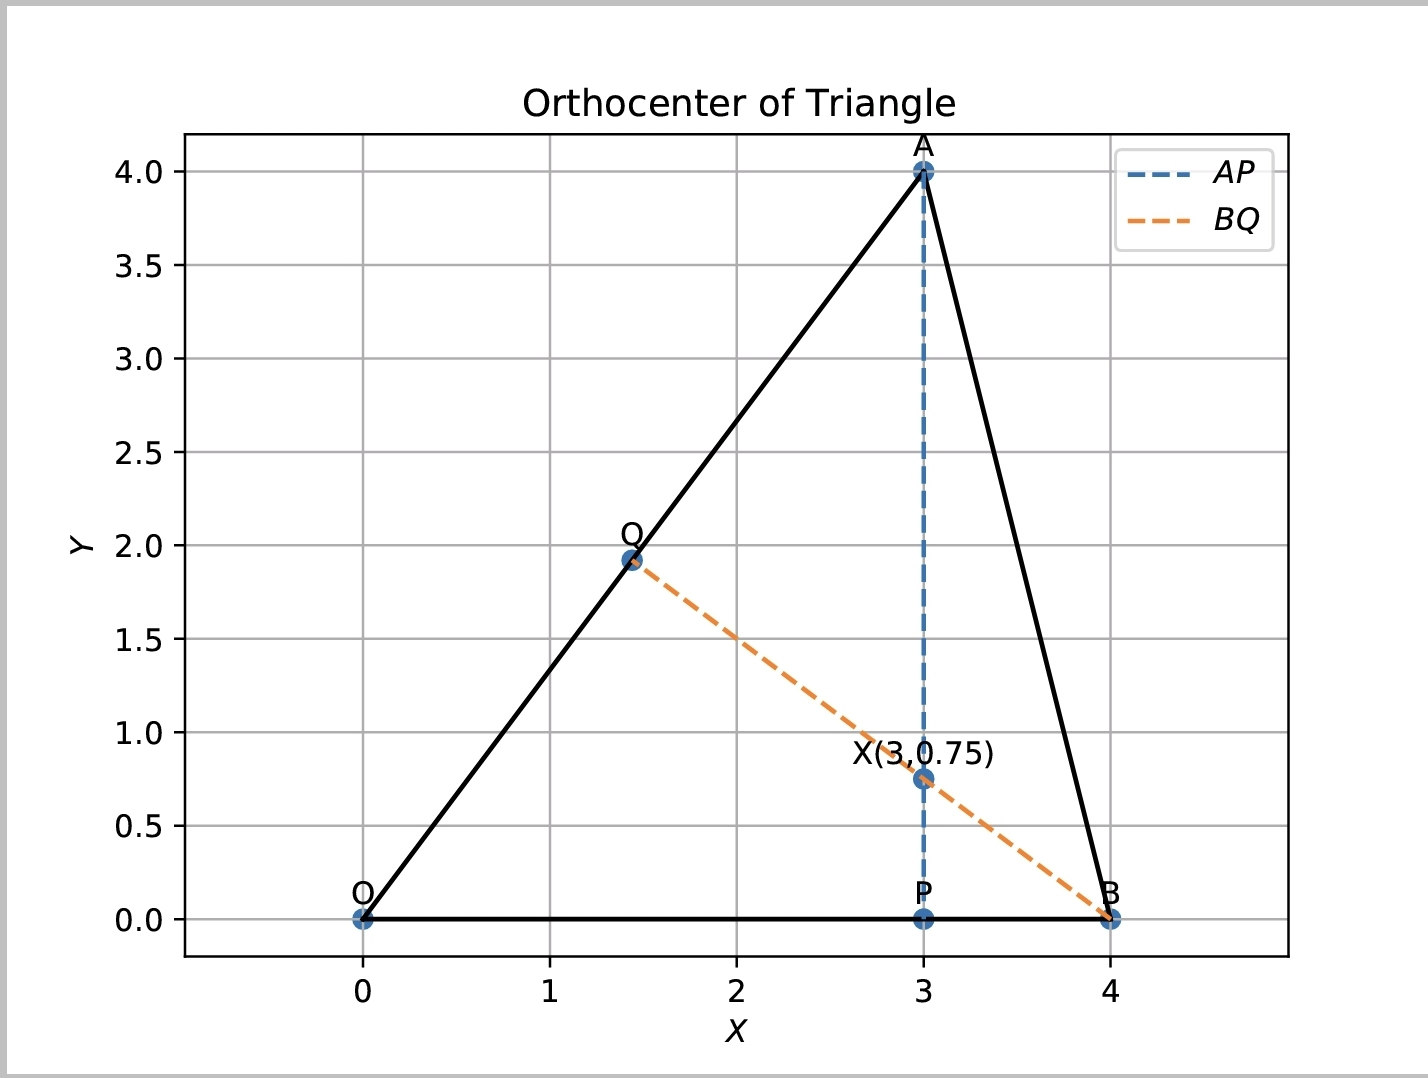
\includegraphics[width=\columnwidth]{fig.jpg}
    \label{fig:my_label}
\end{figure}


\section{\textbf{Code Link}}

\begin{lstlisting}
https://github.com/nikhilnair90/FWC-2/blob/main/Matrix/Line/line.py
\end{lstlisting}
Execute the code by using the command\\
\textbf{python3 line.py}



\end{document}
